\section{Results}
\label{sec:results}

\subsection{Some Results Using Different Images}

The Canny Edge Detector was applied to various images, demonstrating its effectiveness in edge detection. The results are shown in \autoref{fig:lenna_grayscale} to \autoref{fig:car_edge_detected}. Each image is presented in grayscale and with the edges detected using the Canny method.

\begin{figure}[ht]
    \centering
    \begin{subfigure}{0.4\textwidth}
        \centering
        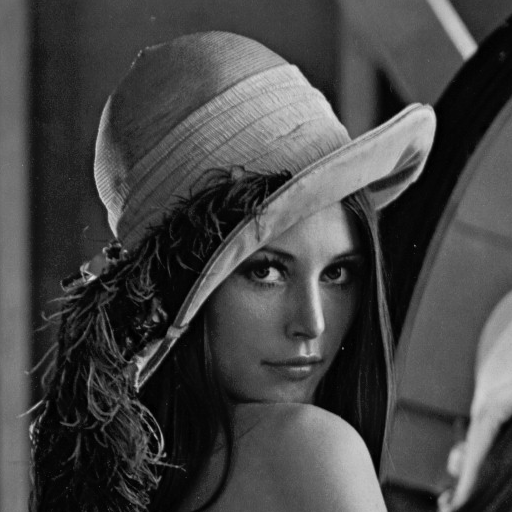
\includegraphics[width=0.9\textwidth]{lenna_2_grayscale.png}
        \caption{Lenna Grayscale}
        \label{fig:lenna_grayscale}
    \end{subfigure}
    \hfill
    \begin{subfigure}{0.4\textwidth}
        \centering
        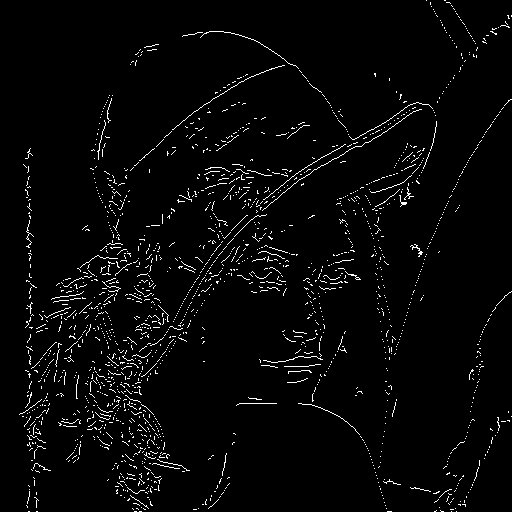
\includegraphics[width=0.9\textwidth]{lenna_8_canny_edge_detected.png}
        \caption{Lenna Edge Detected}
        \label{fig:lenna_edge_detected}
    \end{subfigure}
    \caption{Canny Edge Detection Results for Different Images (Part 1)}
\end{figure}

\begin{figure}[ht]\ContinuedFloat
    \centering
    \begin{subfigure}{0.4\textwidth}
        \centering
        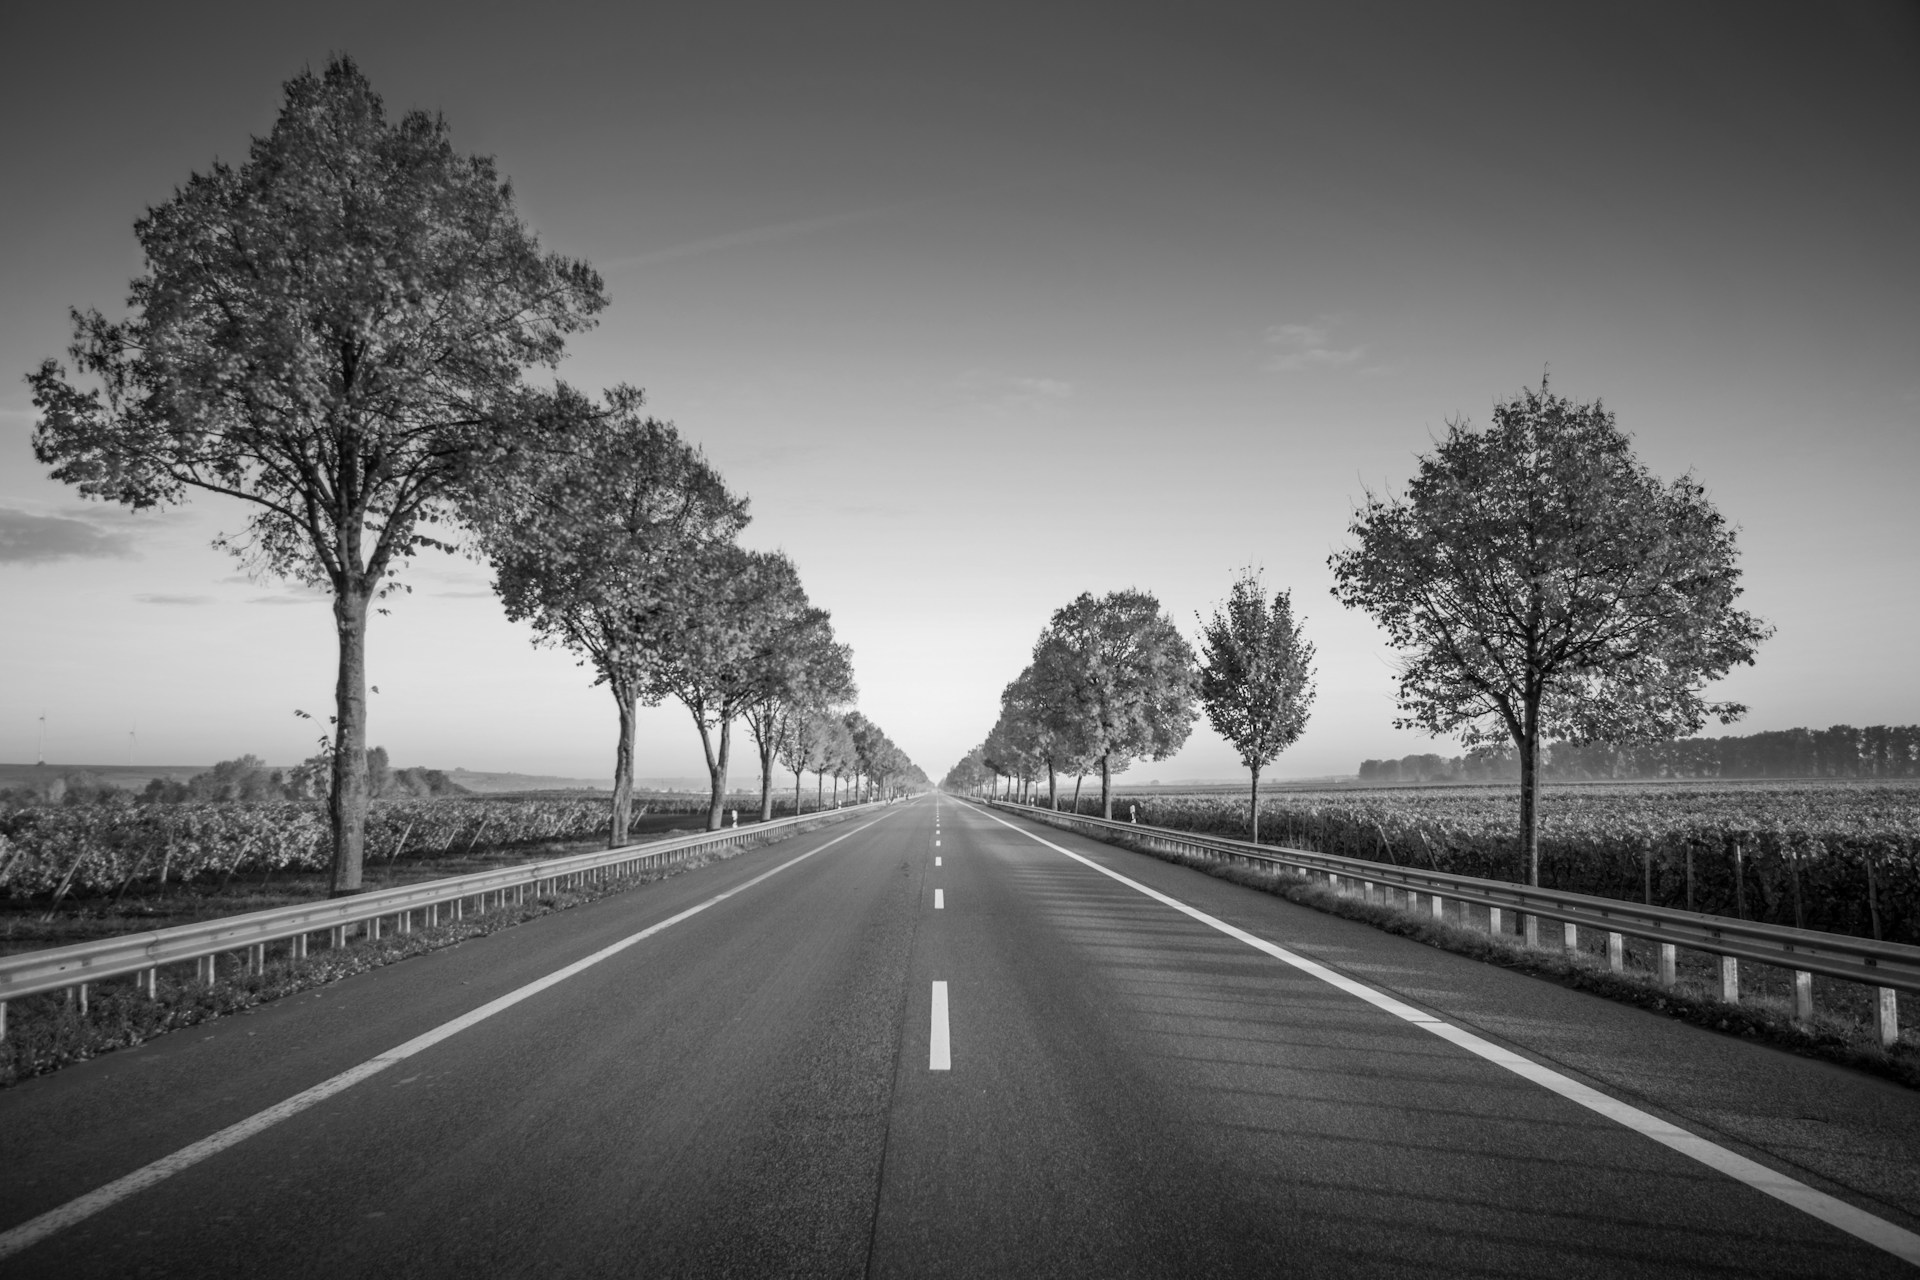
\includegraphics[width=0.9\textwidth]{road_2_grayscale.png}
        \caption{Road Grayscale}
        \label{fig:road_grayscale}
    \end{subfigure}
    % \hfill
    \begin{subfigure}{0.4\textwidth}
        \centering
        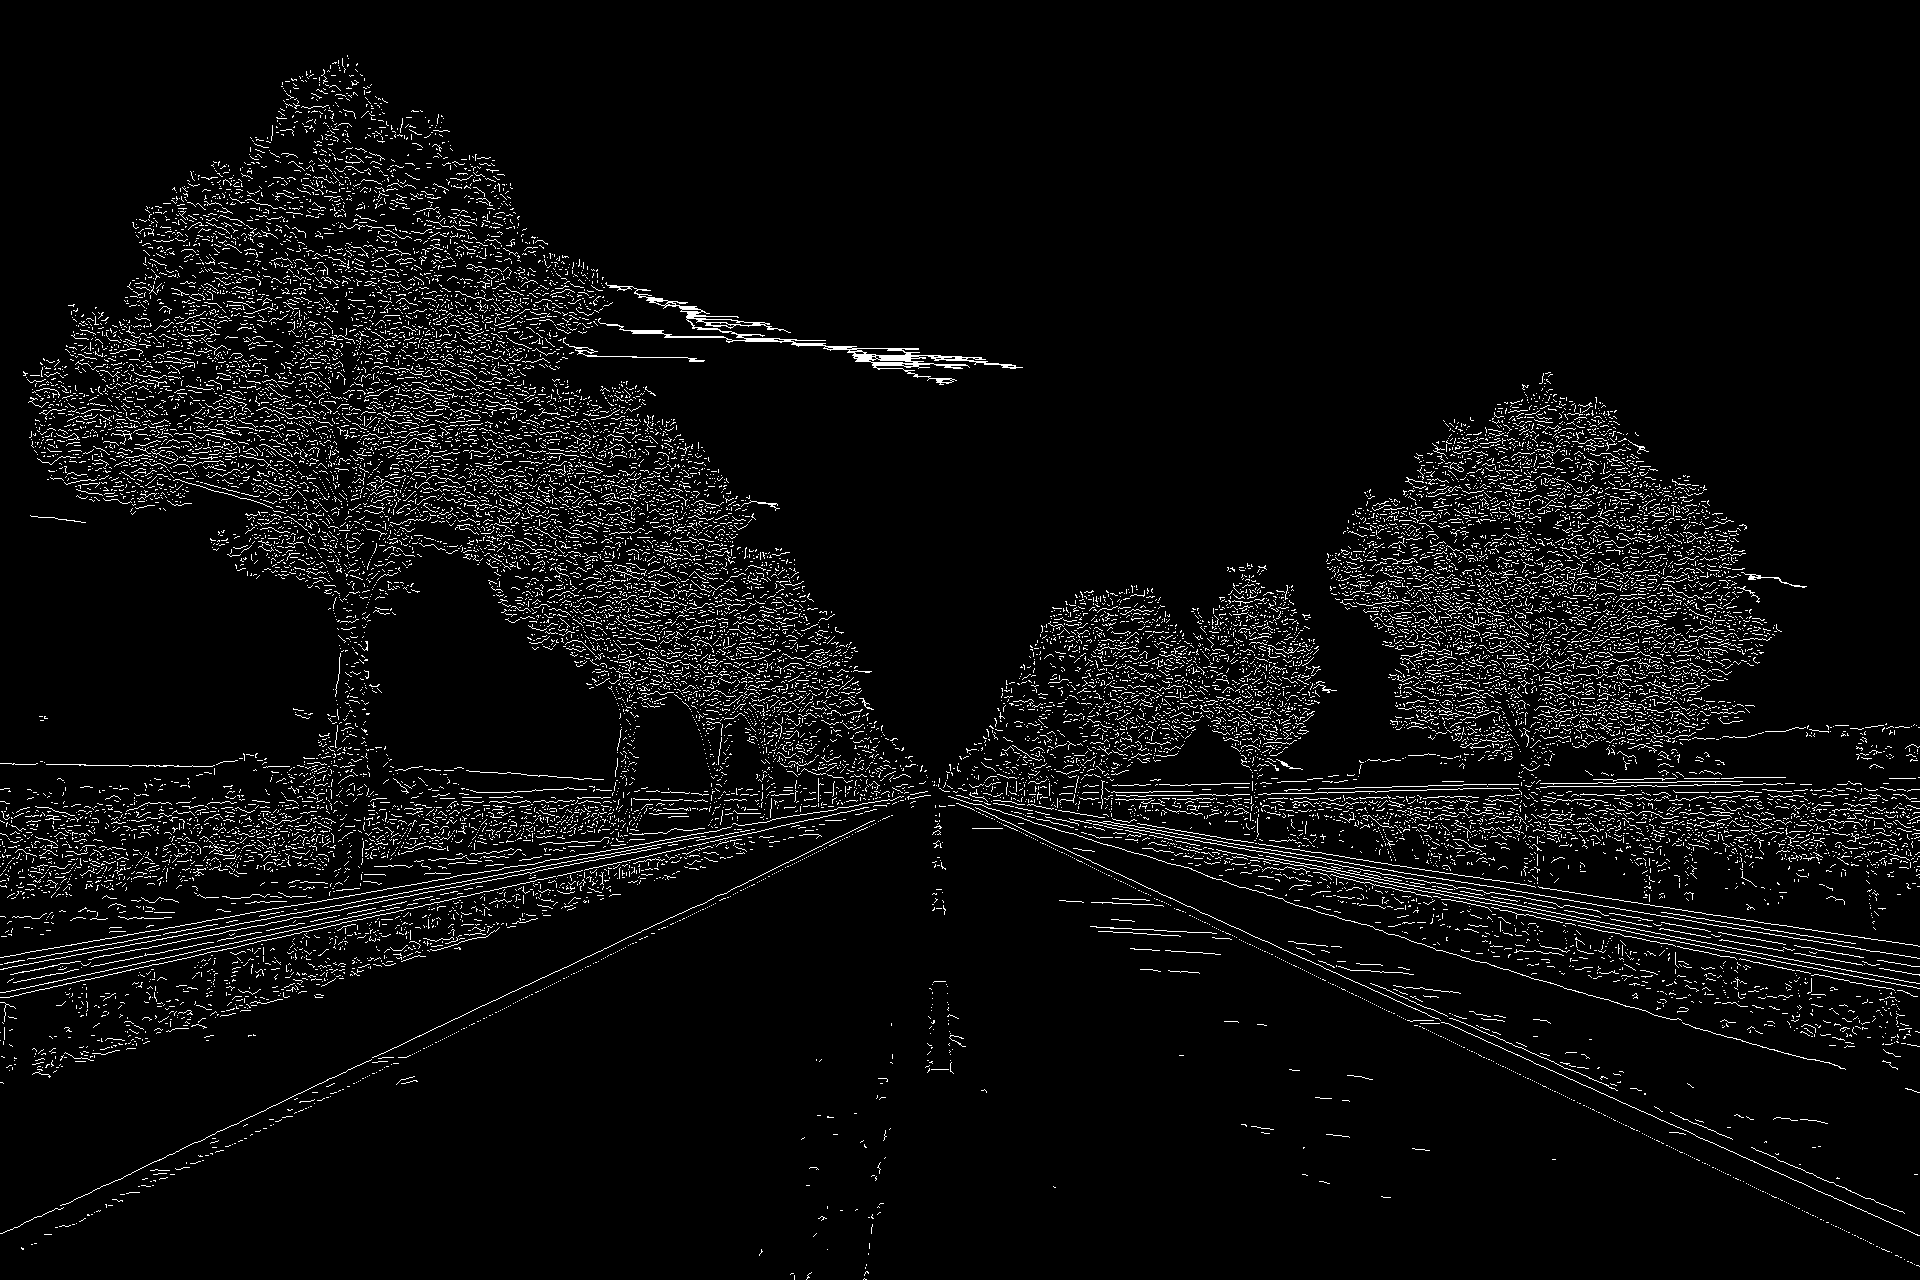
\includegraphics[width=0.9\textwidth]{road_8_canny_edge_detected.png}
        \caption{Road Edge Detected}
        \label{fig:road_edge_detected}
    \end{subfigure}
    \caption{Canny Edge Detection Results for Different Images (Part 2)}
\end{figure}

\begin{figure}[ht]\ContinuedFloat
    \centering
    \begin{subfigure}{0.4\textwidth}
        \centering
        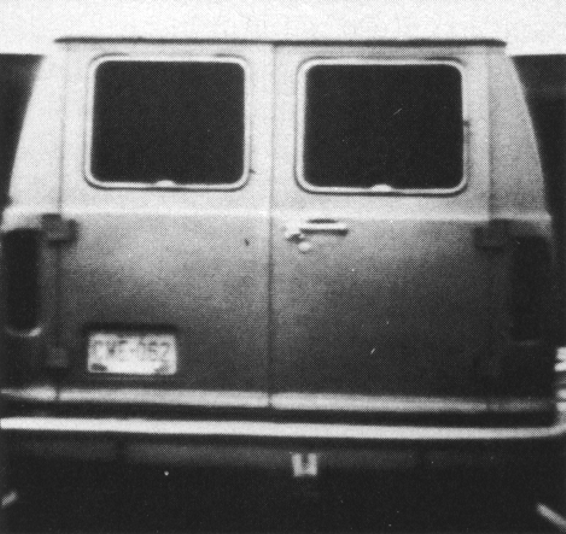
\includegraphics[width=0.9\textwidth]{van_2_grayscale.png}
        \caption{Van Grayscale}
        \label{fig:van_grayscale}
    \end{subfigure}
    % \hfill
    \begin{subfigure}{0.4\textwidth}
        \centering
        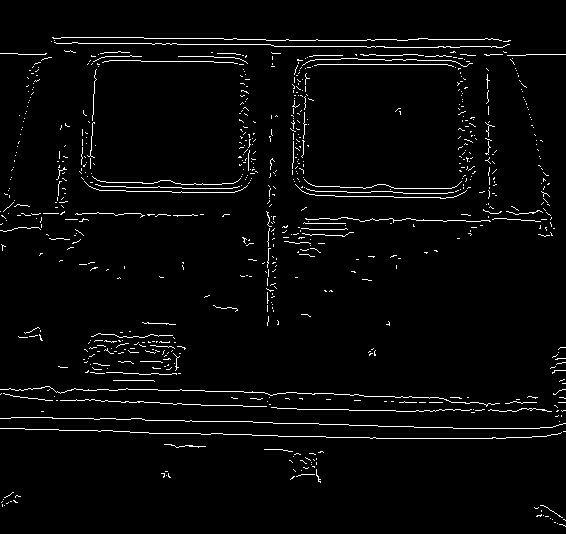
\includegraphics[width=0.9\textwidth]{van_8_canny_edge_detected.png}
        \caption{Van Edge Detected}
        \label{fig:van_edge_detected}
    \end{subfigure}
    \caption{Canny Edge Detection Results for Different Images (Part 3)}
\end{figure}

\begin{figure}[ht]\ContinuedFloat
    \centering
    \begin{subfigure}{0.4\textwidth}
        \centering
        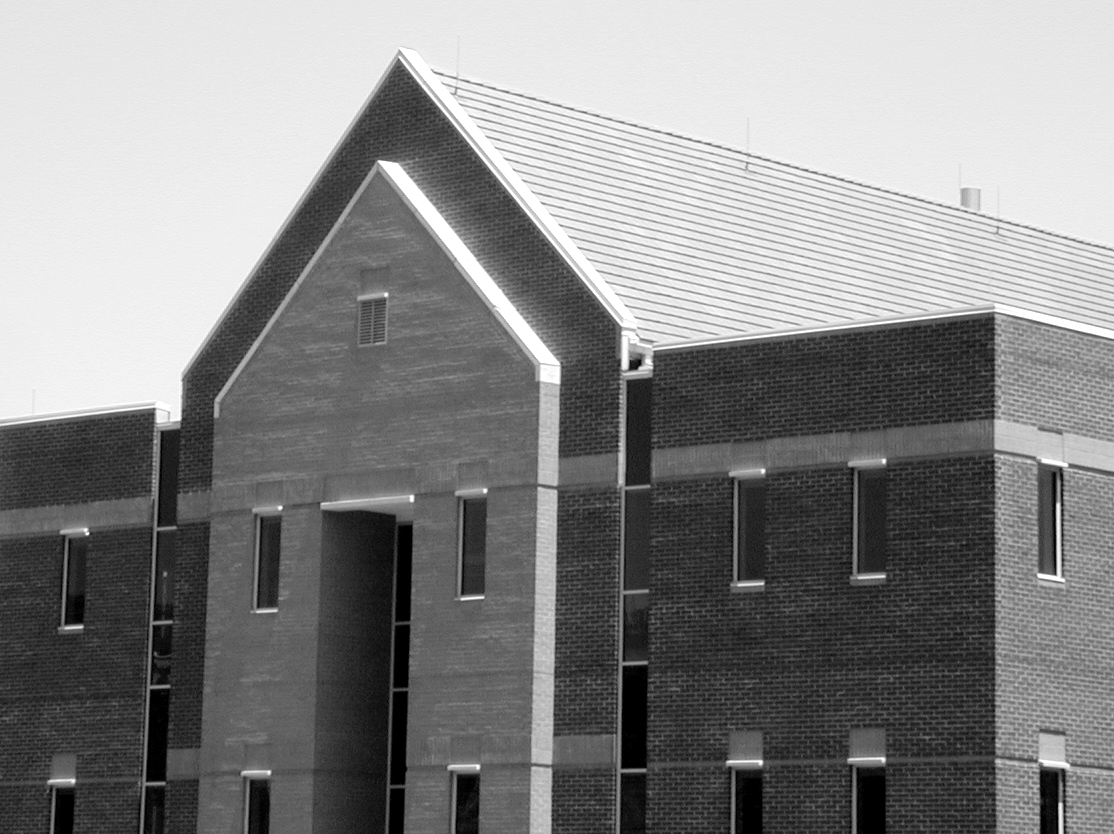
\includegraphics[width=0.9\textwidth]{building_2_grayscale.png}
        \caption{Building Grayscale}
        \label{fig:building_grayscale}
    \end{subfigure}
    \hfill
    \begin{subfigure}{0.4\textwidth}
        \centering
        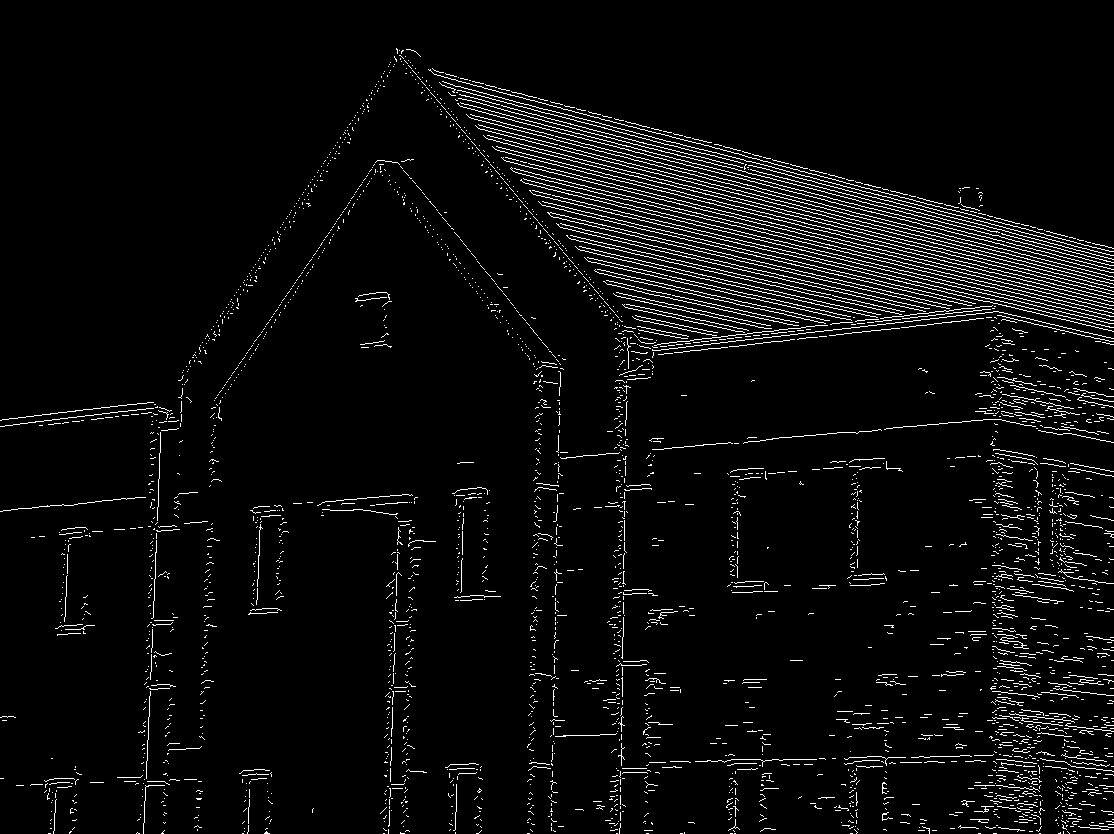
\includegraphics[width=0.9\textwidth]{building_8_canny_edge_detected.png}
        \caption{Building Edge Detected}
        \label{fig:building_edge_detected}
    \end{subfigure}
    \caption{Canny Edge Detection Results for Different Images (Part 4)}
\end{figure}

\begin{figure}[ht]\ContinuedFloat
    \centering
    \begin{subfigure}{0.4\textwidth}
        \centering
        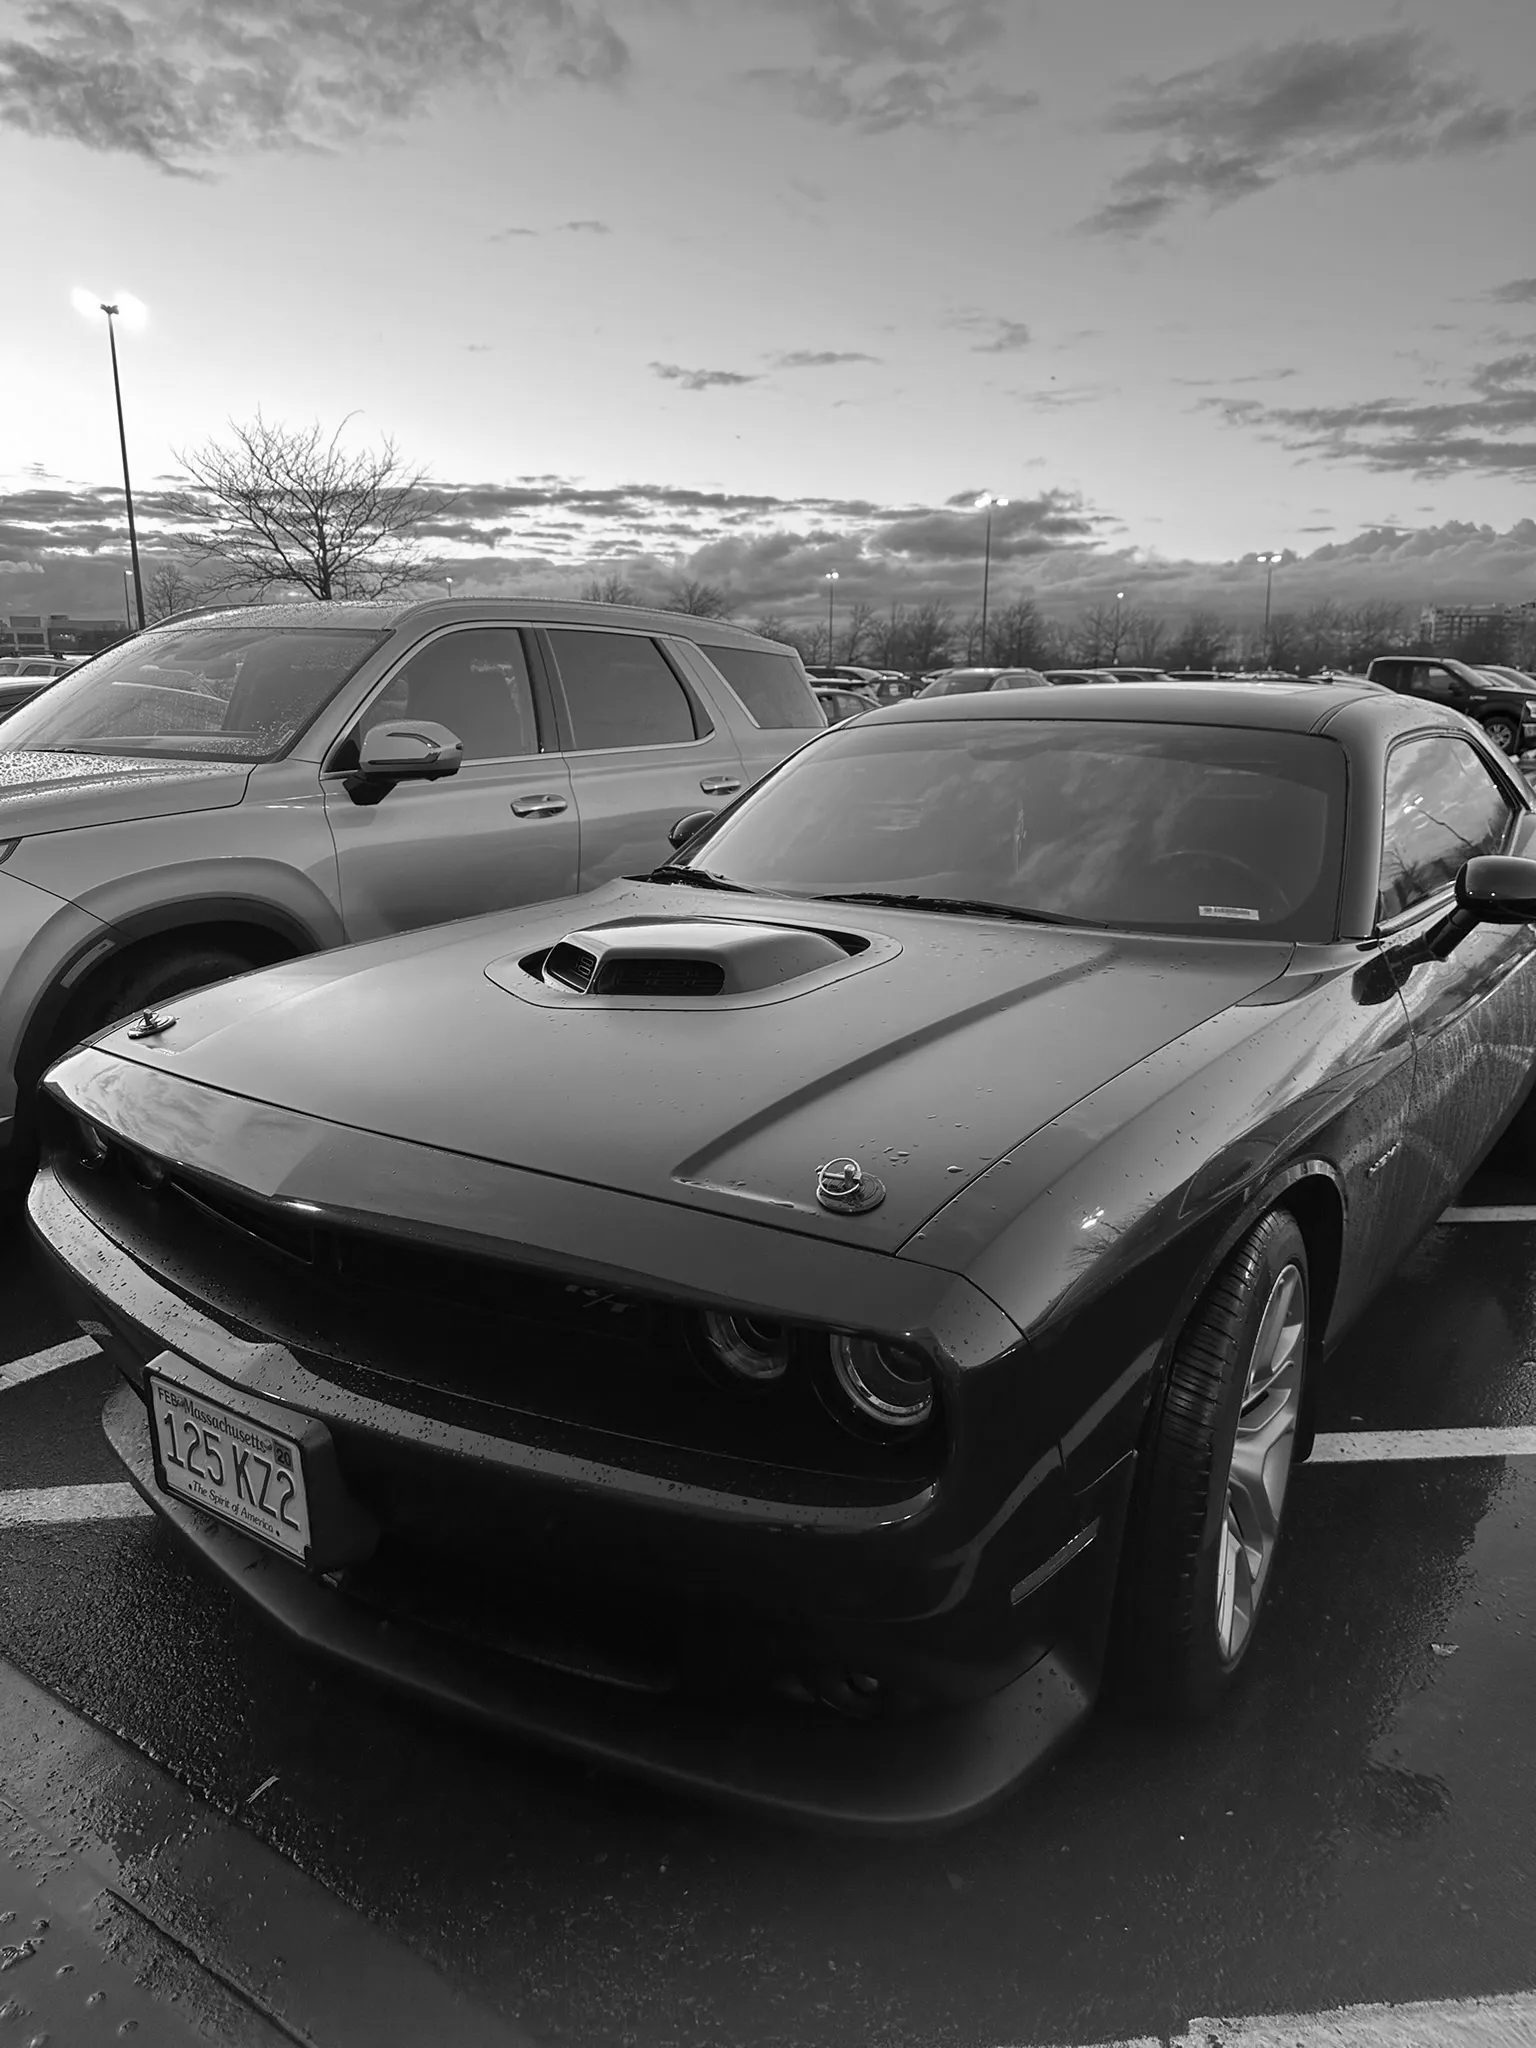
\includegraphics[width=0.9\textwidth]{car_2_grayscale.png}
        \caption{Car Grayscale}
        \label{fig:car_grayscale}
    \end{subfigure}
    \hfill
    \begin{subfigure}{0.4\textwidth}
        \centering
        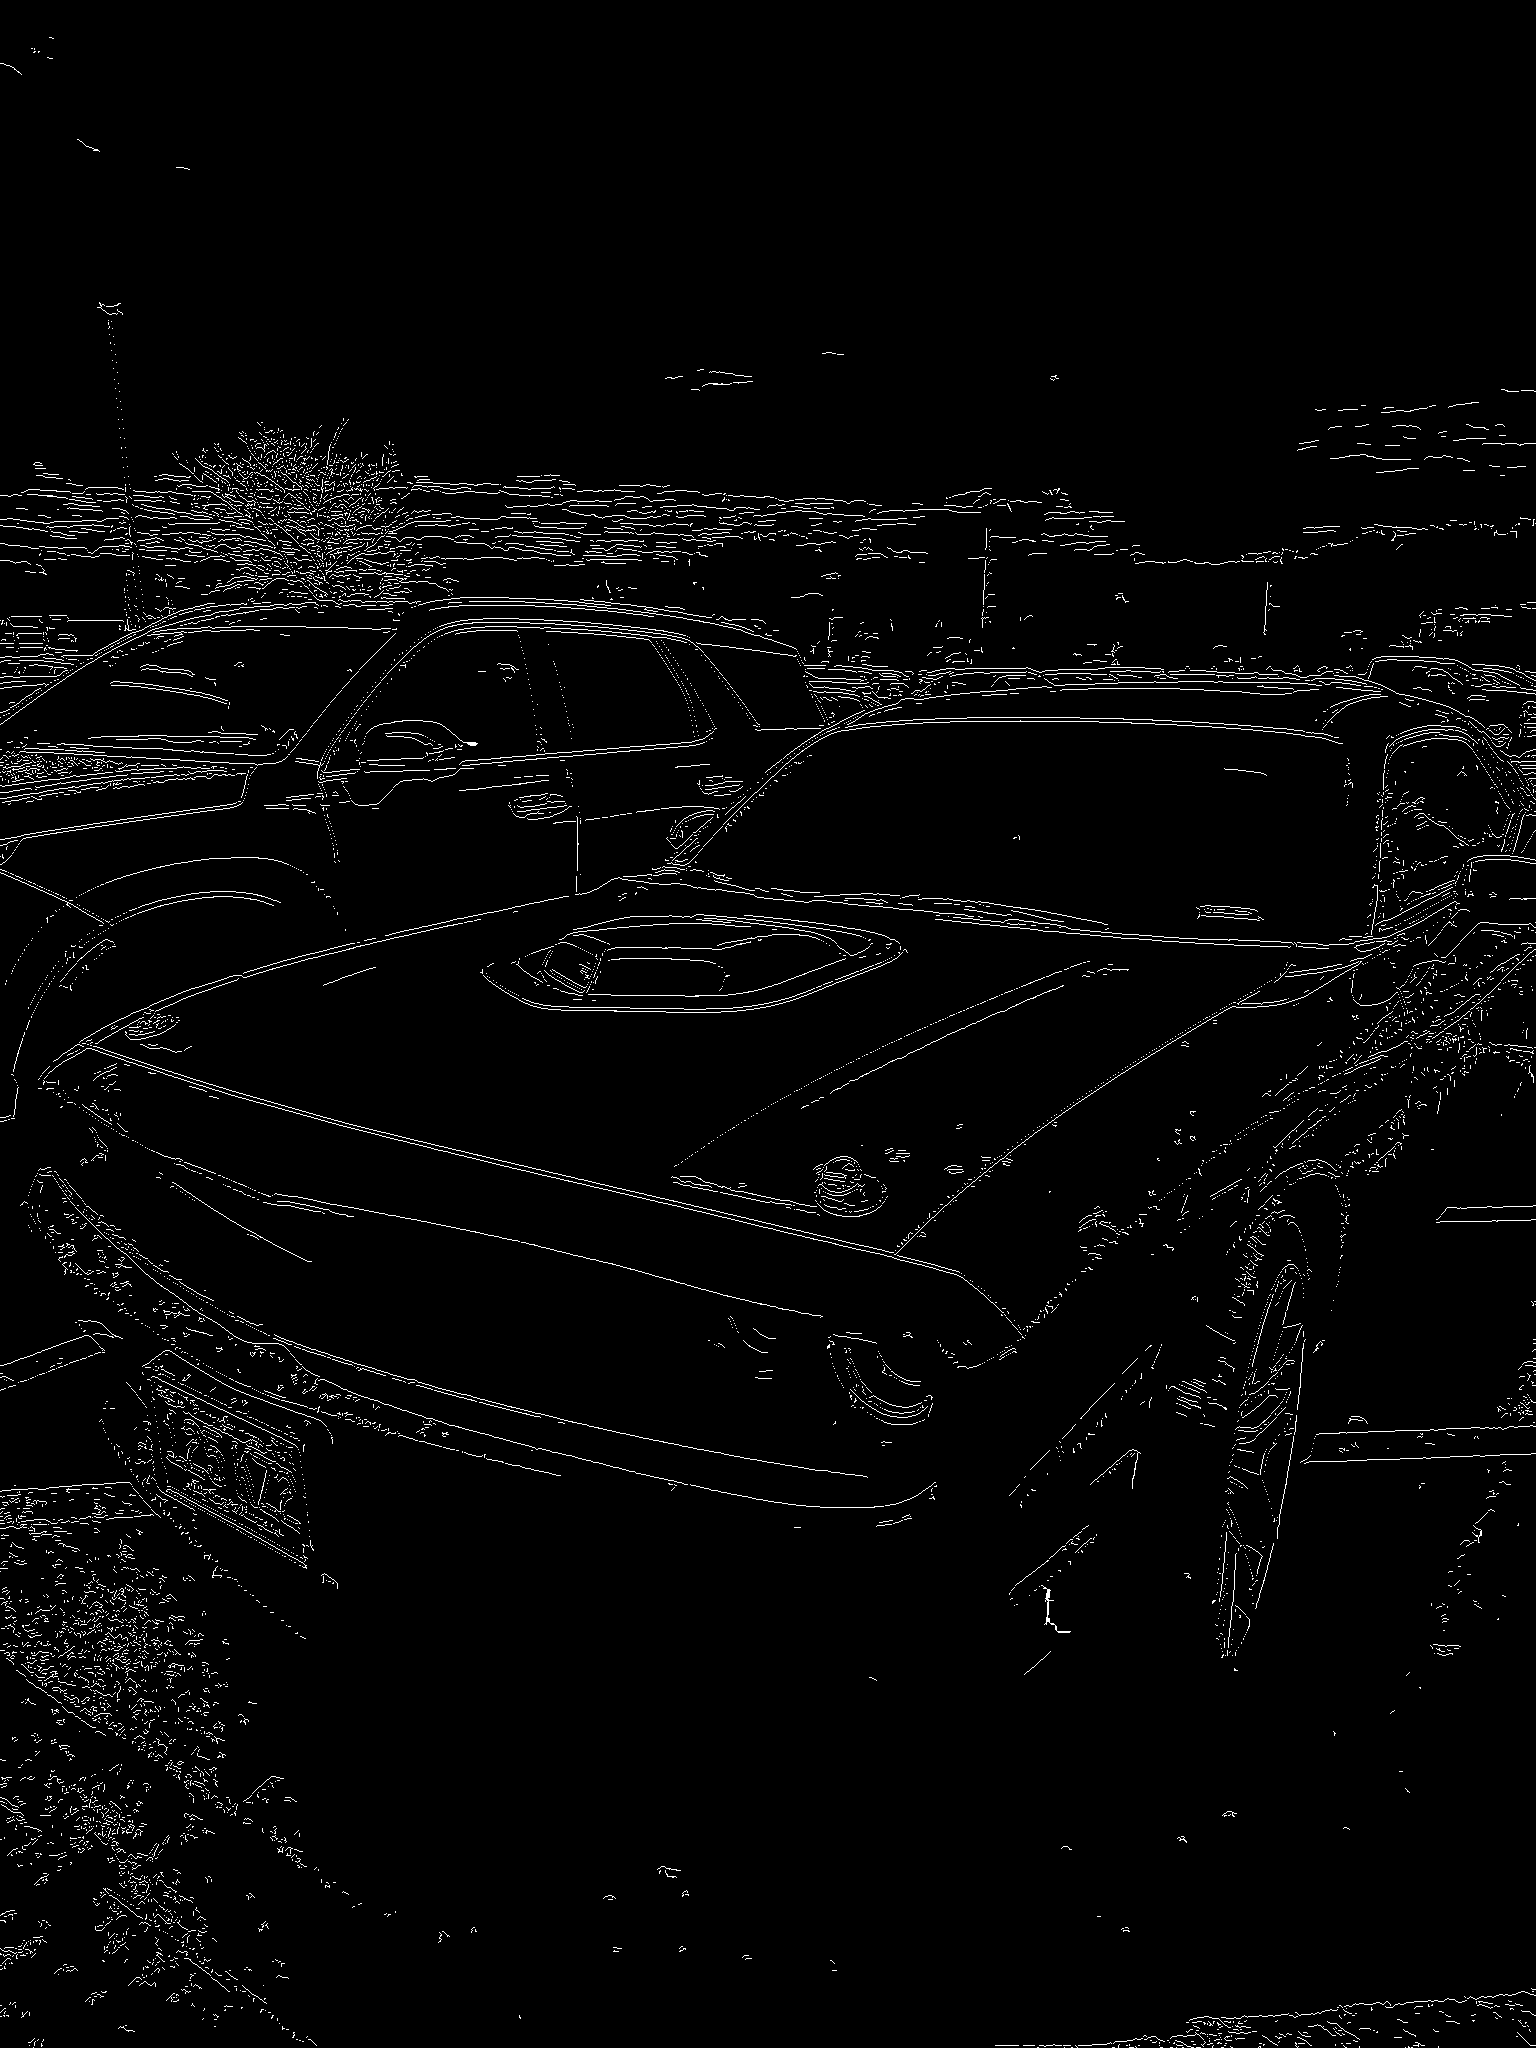
\includegraphics[width=0.9\textwidth]{car_8_canny_edge_detected.png}
        \caption{Car Edge Detected}
        \label{fig:car_edge_detected}
    \end{subfigure}
    \caption{Canny Edge Detection Results for Different Images (Part 5)}
\end{figure}

\clearpage

\subsection{Comparison of Different Thresholds}
The Canny Edge Detector was applied to the same image with different thresholds to observe the effect on edge detection. The results are shown in \autoref{fig:thresholds}.

\begin{figure}[ht]
    \centering
    \begin{subfigure}{0.3\textwidth}
        \centering
        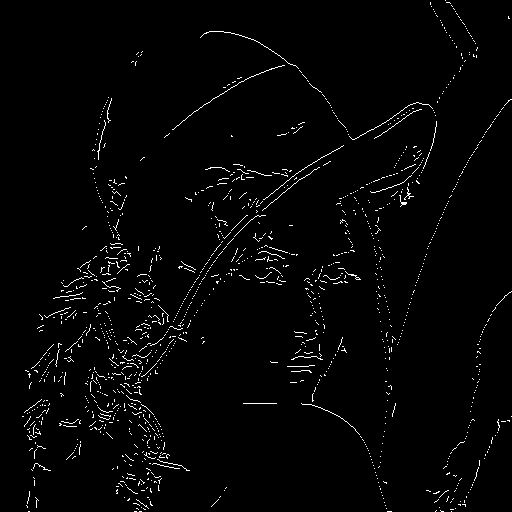
\includegraphics[width=0.9\textwidth]{lenna_8_canny_edge_detected0.01_0.2.png}
        \caption{Thresholds: 0.01, 0.2}
    \end{subfigure}
    \hfill
    \begin{subfigure}{0.3\textwidth}
        \centering
        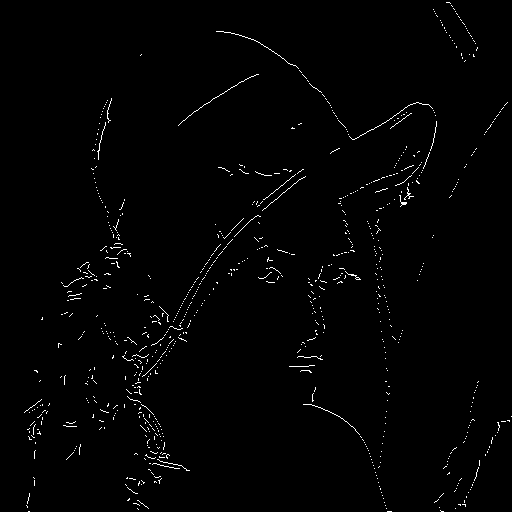
\includegraphics[width=0.9\textwidth]{lenna_8_canny_edge_detected0.01_0.3.png}
        \caption{Thresholds: 0.01, 0.3}
    \end{subfigure}
    \hfill
    \begin{subfigure}{0.3\textwidth}
        \centering
        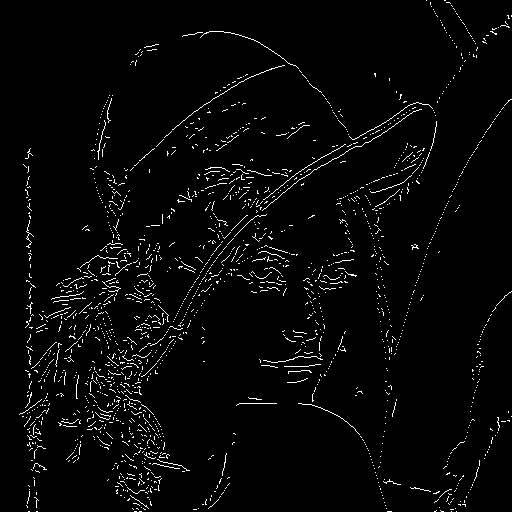
\includegraphics[width=0.9\textwidth]{lenna_8_canny_edge_detected0.1_0.15.png}
        \caption{Thresholds: 0.1, 0.15}
    \end{subfigure}
    
    \vspace{0.5cm}
    
    \begin{subfigure}{0.3\textwidth}
        \centering
        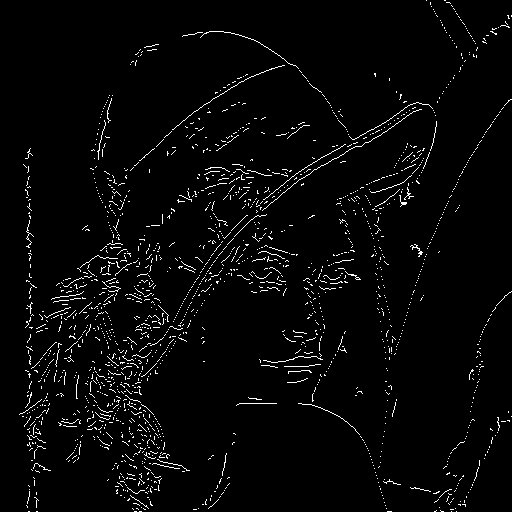
\includegraphics[width=0.9\textwidth]{lenna_8_canny_edge_detected0.01_0.15.png}
        \caption{Thresholds: 0.01, 0.15}
    \end{subfigure}
    \hfill
    \begin{subfigure}{0.3\textwidth}
        \centering
        
\includegraphics[width=0.9\textwidth]{lenna_8_canny_edge_detected0.01_0.25.png}
        \caption{Thresholds: 0.01, 0.25}
    \end{subfigure}
    \hfill
    \begin{subfigure}{0.3\textwidth}
        \centering
        
\includegraphics[width=0.9\textwidth]{lenna_8_canny_edge_detected0.15_0.25.png}
        \caption{Thresholds: 0.15, 0.25}
    \end{subfigure}
    
    \caption{Canny Edge Detection Results with Different Thresholds}
    \label{fig:thresholds}
\end{figure}


% \clearpage